\chapter{Crystal symmetries in group-V monolayers}
\label{ch:oals}
 
What seems to be a natural extension to the ten-fold way is to include spatial symmetries, which are inherently connected to crystalline solids. However, this remains a tedious task due to a large number of possible symmetry configurations (there are 230 space groups in three-dimensions, or 1651 magnetic groups)~\cite{Slager2013, PhysRevB.90.165114, PhysRevB.93.195413, PhysRevB.95.235425, PhysRevB.93.045429}.

The presence of crystalline symmetries gives rise to new topological phenomena. Topological crystalline insulators (TCI) are systems in which gapless boundary modes are solely protected by the spatial symmetries. For instance, in the semiconducting bulk SnTe two-dimensional surface states are protected by the mirror symmetry~\cite{FuTCI2011, HsiehTCI2012} acting non-locally in a real space. Another prominent consequence is the concept of higher-order topological insulators, where non-trivial $d$-dimensional bulk is accompanied by boundary modes in a $(d-n)$ dimensions, with $n > 1$~\cite{Benalcazar61, PhysRevLett.119.246401, HOTI12018}. 

A unifying framework of topological quantum chemistry~\cite{TQC2017} provides a classification based on group theory and local atomic orbitals.






\section{Topological crystalline insulating states in two-dimensional monolayers}

Despite recent theoretical developments including TCI protected by rotation~\cite{PhysRevX.9.031003, Fangeaat2374}
there are not many material candidates for TCI  (planar Bi/Sb with DFT~\cite{Hsu2016}),  electron-doped TlM (M = S and Se) (110) monolayer~\ref{Niu2015}, monolayer and trilayer PbTe~\cite{C7CP04679K}.

\subsection{Liu-Allen tight-binding model}
We employ $sp^3$ tight-binding model developed in Ref. \cite{Liu:Allen} for bulk bismuth and antimony, neglecting hoppings between bilayers as proposed in Ref. \cite{Murakami:BiQSH}. Interatomic hoppings are parametrized within the Slater-Koster approach \cite{Slater:Koster} and atomic spin-orbit coupling $\lambda \vec{L}\cdot\vec{S}$. The Hamiltonian of the model reads
\begin{equation}
\begin{aligned}
&H = \sum_{i, \alpha,\sigma}E_{i\alpha}c^\dagger_{i\alpha\sigma}c_{i\alpha\sigma} +\sum_{i,\alpha,\sigma}E_{Field}^{R,G}c^\dagger_{i\alpha\sigma}c_{i\alpha\sigma}  \\
& + \left[ \sum_{i,j,\alpha,\alpha',\sigma}V_{\alpha\alpha'}c^\dagger_{i\alpha\sigma}c_{j\alpha'\sigma} +\frac{\lambda}{3}\sum_{i}(c^\dagger_{iz\downarrow}c_{ix\uparrow} - c^\dagger_{iz\uparrow}c_{ix\downarrow} \right. \\
& \left. +ic^\dagger_{iz\uparrow}c_{iy\downarrow}+ic^\dagger_{iz\downarrow}c_{iy\uparrow} +ic^\dagger_{ix\downarrow}c_{iy\downarrow}-ic^\dagger_{ix\uparrow}c_{iy\uparrow})+ H. c. \right] ,
\end{aligned}
\label{eq:liu allen}
\end{equation}
where $i, j$ are lattice indices, $\alpha = \lbrace s, p_x, p_y, p_z \rbrace$ labels orbitals an $\sigma= \lbrace \uparrow,\downarrow \rbrace$ denotes spins. $E_{i}$ corresponds to the on-site energies and $V_{\alpha\alpha'}$ are the hopping integrals. $E_{Field}^{R} =-E_{Field}^{G} =E_{Field}$ is a perpendicular electric field on $i\in R$ and $i\in G$ sites of two sublattices in a lattice indicated by red and green color in Fig. \ref{fig:latt_struct}. The last term is the SOC with a strength $\lambda$. According to Chadi \cite{Chadi}, 1/3 factor is introduced to renormalized atomic SOC in order to obtain correct SOC splitting of the valence band. 

\begin{table}
\centering
\begin{tabular}{|c|c|c||c|c|c|}
\hline 
Parameter & Bi & Sb & Parameter  & Bi & Sb \\ 
 (eV) &  &  & (eV)  &  &  \\ \hline
E$_{s}$ & -10.906 & -10.068 & V'$_{sp\sigma}$ & 0.433 & 0.478 \\ 
E$_{p}$ & -0.486 & -0.926 & V'$_{pp\sigma}$  & 1.396 & 1.418  \\
V$_{ss\pi}$ & -0.608 & -0.694 & V$'_{pp\pi}$ & -0.344 & -0.393 \\
V$_{sp\sigma}$ & 1.320 & 1.554 & V''$_{ss\sigma}$ & 0 & 0 \\
V$_{pp\sigma}$ & 1.854 & 2.342 & V''$_{sp\sigma}$ & 0 & 0\\
V$_{pp\pi}$& -0.600 & -0.582 & V''$_{pp\sigma}$ & 0.156 & 0.352 \\
V'$_{ss\sigma}$& -0.384 & -0.366 & V''$_{pp\pi}$ & 0 & 0\\
$\lambda$ & 1.5 & 0.6 &   & & \\
\hline
a ($\textnormal{\AA}$) & 4.53 & 4.30 & h ($\textnormal{\AA}$) & 1.58$^{*}$ & 1.64$^{**}$ \\
d$_1$ ($\textnormal{\AA}$) & 3.062 & 2.902 &  &  &\\
\hline
\end{tabular} 
\caption{Tight-binding parameters for Bi and Sb taken from Refs. \cite{Liu:Allen}, \cite{stable:bi111}$^*$, \cite{Sb:nontriv}$^{**}$. $d_1$ denotes nearest-neighbor distance between sites in a honeycomb lattice.}
\label{tab:TB}
\end{table}

Similarities between Bi and Sb crystals can be seen by looking at Slater-Koster parameters listed in Table I, taken from Ref. \cite{Liu:Allen}. Most of the parameters differ by less than $15\%$. The only significant change is in the spin-orbit coupling constant $\lambda$, $2.5$ times larger in bismuth. Thus, a transition from QSH insulating phase to trivial insulator with increasing $x$ in Bi$_{1-x}$Sb$_x$ is related, in general, to a decrease of spin-orbit coupling constant.


\subsection{Mirror Chern number}

For the case of mirror, the 3Dspace is split in two regions by the mirror plane on whichmirror symmetry acts as an internalZ2symmetry.  Thissymmetry can be used to transform the Hamiltonian intoa block-diagonal form where the two blocks are relatedby time-reversal symmetry.  Each block separately maybreak  time  reversal  symmetry  (class  A),  hence,  we  canassign to it a non-vanishing Chern numberCcorrespond-ing to a quantum Hall or Chern insulator phase (the totalChern number of the two blocks is still zero).  The result-ing TCI is characterized by mirror Chern numberCinthe corresponding mirror plane.

When $d_z = 0$, a mirror symmetry $M_z$ is restored and TCI phase is exhibited. Recall that mirror Chern number is defined as a difference between Chern numbers corresponding to different mirror-symmetric subsystems:
\begin{equation}
\mathcal{C} = \frac{C_{+ M} - C_{-M}}{2}
\label{eq:mirror_chern}
\end{equation}

\subsection{Entanglement measures}

\subsubsection{Entanglement entropy}
The concept of the Shannon entropy of a statistical distribution can be extended to the quantum case by defining an entanglement entropy 
\begin{equation}
S( \rho) = -Tr (\rho \log \rho) = \sum_i \lambda_i \log \lambda_i
\end{equation}
$\lambda_i$ are the eigenvalues of $\rho$ (with the assumption that $0 \log 0 \equiv 0$).


\subsubsection{Entanglement spectrum}
Calculating entanglement entropy gives a particular number. Therefore, Li and Haldane proposed that the full eigenvalue spectrum of the reduced density matrix may be used to distinguish between phases. This concept has been applied to topological in- sulators, quantum spin chains or quantum Hall fluids. Due to the positivity and Hermiticity, the reduced density matrix $\rho_A$ can be written as follows
\begin{equation}
\rho_A = \frac{1}{Z} e^{-H_{ent}}
\end{equation}
with the partition function $Z = Tr \exp (-H_{ent})$. Hent is the entanglement Hamiltonian and the eigenenergies of Hint are called entanglement spectrum. Thanks to this form of density matrix, the entanglement entropy can be considered as an equivalent to the thermodynamic entropy with a Hamiltonian Hent at temperature T = 1. For a weak entanglement, the gap in spectrum of Hent separates ground state eigenvalue from ’excited states’. In the limit of no entanglement within the system, the gap becomes infinite. A remarkable insight has been made for topological phases in 2 + 1-dimensions, known as an edge-entanglement spectrum correspondence. If the system has edge states (or, in general, possesses low-energy states near an open boundary of the manifold where the system lives), the low-lying edge spectrum of the physical boundary Hamiltonian is an one-to-one correspondence with the low-lying spectrum of Hent

\subsubsection{Free-fermionic systems}
Entanglement measures for free fermionic lattice systems can be computed from the two-point correlation function restricted to the subsystem \cite{Peschel}
\begin{equation}
C^{\alpha \beta}_{ij}= \textnormal{Tr} \left( \rho_A c^{\dagger}_{i\alpha} c_{j\beta} \right),
\end{equation}
where $i, j$ are lattice indices within the subsystem $A$ and $\alpha, \beta$ label orbitals or spins. If system is translationally-invariant, the Hamiltonian $H$ can be written in the momentum space with the many-body ground state in a form $\ket{GS} = \prod_{n, k}  a^{\dagger}_{n k} \ket{0}$ with operators $a^{\dagger}_{n k}$ corresponding to creation a particle with momentum $k$ and $n$ running over the occupied single-particle Bloch states. Hence, the correlation matrix can be evaluated for each $k$-point separately via formula $C^{\alpha \beta}_{ij} (k) = \braket{GS | c^{\dagger}_{i\alpha k} c_{j \beta k} | GS}$. $C(k)$ is a Hermitian matrix and can be regarded as a spectrally flattened physical Hamiltonian with eigenvalues (denoted by $\lbrace \zeta_k \rbrace$) falling between $0$ and $1$. Most of the eigenvalues in the spectrum of $C(k)$ lie exponentially close to either 1 or 0, depending whether bulk states are fully localized in the subsystem $A$ or $B$, respectively, and do not contribute to the entanglement entropy. However, states crossing the partition boundary give rise to non-zero entanglement entropy. If the Hamiltonian describes a topologically non-trivial $Z_2$ phase in 2D, $C(k)$ will reveal the spectral flow associated with continuous set of intermediate eigenvalues \cite{Hughes:inv, Vish:inv}. A relation between $\lbrace \zeta_k \rbrace$ and the spectrum of $H_A(k)$ labeled by $\lbrace \xi_k \rbrace$ is following
\begin{equation}
\zeta_k = \left( 1+e^{\xi_k} \right)^{-1}.
\end{equation}
Due to this one-to-one correspondence, we refer to eigenvalues of the correlation matrix as the single-particle entanglement spectrum, which is a conventional practice in the literature \cite{Alex:CM, Vish:inv, Hughes:inv}. Entanglement entropy is then given by
\begin{equation}
S_A = - \sum_a \left( \zeta_a \log \zeta_a + \left( 1 - \zeta_a \right) \log \left( 1 - \zeta_a \right) \right),
\label{eq:entCij}
\end{equation}
where $a$ is index running over all eigenvalues of $C$. $S_A$ can be calculated \cite{Ryu:EE} by summing over the entanglement entropy for each $k$-point with a normalization factor being the number of unit cells $S_{A} = 1 / N_y \sum_k S_A(k)$.

The number of intersecting branches of edge states in the band structure allows us to distinguish between TI and TCI phases. Similar features can be also observed in entanglement spectra.



\subsection{Free-standing layers }
\subsection{Substrate effect }
only one pair of modes spectrally connecting 0’s and 1’s is noticed. Hence, we can identify these spectra with TI phase. In order to realize TCI phase in these systems, one needs to find a substrate that weakly couples.


\section{Obstructed atomic limits}
n  general,  a  set  of  occupied  bands  (without  strong  orfragile  topology)  can  be  decomposed  into  subsets  of  bandsstemming from localized orbitals at different Wyckoff posi-tions. The minimal subblocks that cannot be further decom-posed  areelementary  band  representations(EBRs),  whichare  a  connected  set  of  subbands  induced  from  placing  acertain  orbital  at  a  given  Wyckoff  position  .A central statement of TQC is that whenever a set of bands has symmetry properties thatare not compatible with the ones of a sum of EBRs, these bands are topological.  In fact, itmeans they cannot be adiabatically connected to an atomic limit with localized orbitals atlattice sites. he topology of a group of bands is entirely character-ized by the symmetry data vectorBcontaining the multiplicity of the various irreduciblerepresentations at different HSPs. Any band structure with symmetry dataBthat satisfies the compatibility relations can always be written as alinear combination of EBRs:

\begin{equation}
B = \sum_i p_i \mathrm{EBR}_i
\end{equation}
where EBRiis the symmetry data vector of theithEBR of the group under consideration,.This decomposition in not generically unique. 


\subsection{Wannier representation}

For Chern insulators it has been shown that a nonzero Chern number presents a topological obstruction that prevents the construction of exponentially localized WFs~\cite{Thouless_1984, PhysRevB.74.235111} (the opposite statement was proved as well~\cite{PhysRevLett.98.046402}). In case of $Z_2$, there is a topological obstruction only if gauge is chosen in a way that time-reversal symmetry is preserved and Wannier functions come in time reversal symmetric pairs~\cite{PhysRevB.83.035108}.

If system has crystal symmetries as well, obstructions to the Wannier representation does not always guarantee stable topology~\cite{PhysRevLett.121.126402}. There may be systems of an intermediate topological stability, which are characterized by a trivial topological index, but they are not topologically equivalent to a fully insulating limit.



Instead, bands may exhibit a fragile topology which is related to the systems that admit Wannier representation, but may be trivialized to an atomic limit (that is, fully insulating limit) by adding degrees of freedom. Two dimensional fragile topological insulators can feature boundary states interpolating between conductance andvalence  bands.  These states,  however,  lack the  robustness of the analogous states in stable topological insulators.Namely, they can be gapped by edge perturbations that preserve the underlying crystalline symmetry.





Surprisingly, a notion of atomic limit becomes not unique - there may be a situation in which the Wannier centers do not coincide with atomic positions (as in the case of trivial atomic limit), but they are rather localized on other symmetric points in the unit cell called the Wyckoff positions.



\begin{figure}
\centering
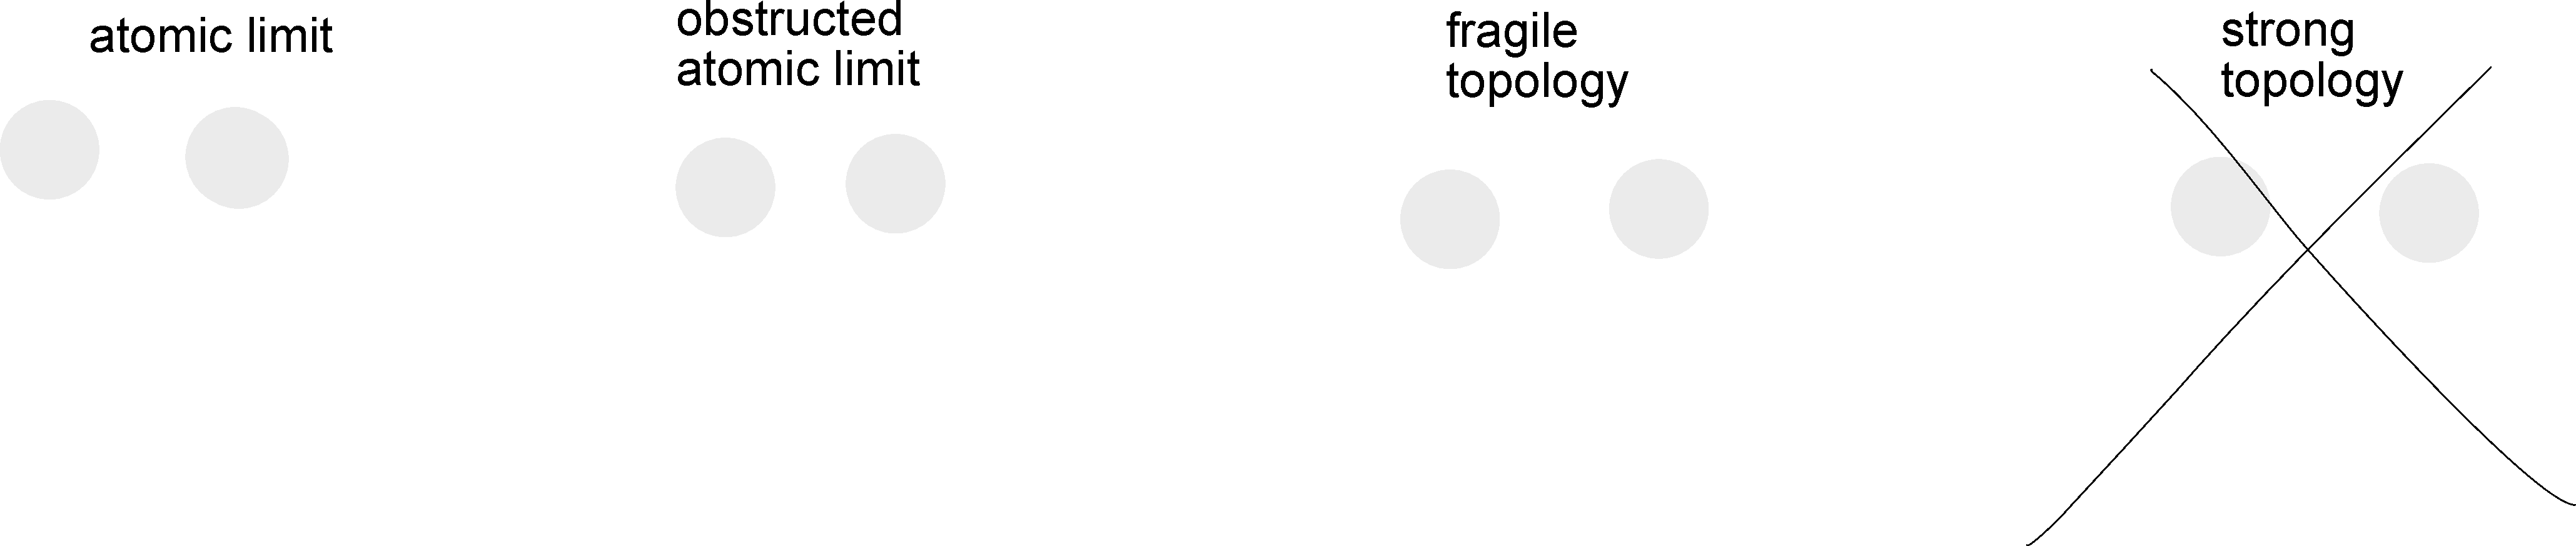
\includegraphics[width=\columnwidth]{oal_newphases}
\caption{In the presence of crystal symmetries, a distinction between topological and trivial phases is less pronounced. Atomic limit corresponds to the situation where Wannier charge centers are located on atomic positions. In case of obstructed atomic limits, Wannier functions are exponentially localized on the Wyckoff positions. Fragile phases cannot be represented in terms of Wannier functions, but a strong index vanishes. Strong topological phases (such as TI or CI) do not admit Wannier representation.}
\label{fig:newphases}
\end{figure}

Quantized  fractional  corner  charges  have  been  predicted  as  a  possible  spectral  signature  for  fragile  topologicalinsulators in the electronic domain.  In a charge neutral system, modes strongly localized at the corners are the counterpart of corner charges.


\subsection{Bulk indices}
The key goal was to construct the bulk indices for all layer groups to be sure that boundary effects are related to the nontrivial bulk rather than suitable edge termination.



\subsubsection{Symmetry indicators}
The Fu-Kane parity criterion for inversion-symmetric topological insulators given in Eq.~\ref{ch:topo-intro} is a special case of more general framework of symmetry indicators~\cite{Po2017}. Band topology is defined b, with a further extension to superconductors~\cite{PhysRevResearch.1.013012}. Symmetry indicators are particularly suitable in a search for real materials as they can be easily employed for ab initio results.

Topological band structures arise whenever there is a mismatch between momentum-space and real-space solutions to symmetry constraint




\subsubsection{Wilson loops}
Non-trivial topology can be captured by the Berry phases of the bands under consideration.  Non-Abelian Wilson loops are a generalization of Berry phase for multi-band system
\begin{equation}
W[\gamma] = \bar{\exp} \left( \oint_{gamma}  d \ell A (\mathbf{k}) \right)
\label{eq:wilson2}
\end{equation}
where $ \bar{\exp}$  path ordering such that operators at the beginning ofthe path appear to the right of operators at the end. 
\begin{equation}
W_{\gamma} = \prod_{\mathbf{k}} P ( \mathbf{k}) 
\label{eq:wilson}
\end{equation}

The Wilson loop operator satisfies $W_\gamma W_\gamma^\dagger = P(\bs{k}^*)$ and so, since any projector satisfies $[P(\bs{k})]^2 = P(\bs{k})$, its eigenvalues are either zero or of the form $e^{\mathrm{i} \theta_\alpha^\gamma}$, $\alpha = 1 \dots N$. In the following, we refer to the set of $\{\theta_\alpha^\gamma\}_{\alpha = 1 \dots N}$ as the Wilson loop spectrum, suppressing the zero eigenvalues. The phases of these eigenvalues (Wilson spectrum) are related to the spectrum of the position operator projected on the space of bands below the gap~\cite{PhysRevB.89.155114}.
Wilson loops can be computed efficiently numerically by employing a discretized version:
\begin{equation}
W [ \gamma] = F_{\mathbf{k}_0, \mathbf{k}_1}  F_{\mathbf{k}_1, \mathbf{k}_2} \ldots  F_{\mathbf{k}_{p-1}, \mathbf{k}_p}
\label{eq:wilson_discretized}
\end{equation}
with $\mathbf{k}_0 = \mathbf{k}_p$ and $F_{\mathbf{k}_i, \mathbf{k}_j}^{m,n} = \braket{u_{\mathbf{k}_i, m} | u_{\mathbf{k}_j, n}$. It is clear how Wilson loops can be regarded asmatrices that map a starting pointk0in momentum space to another point along the loop under parallel transport

The eigenvalues of $W$ along any non-contractible loop $\gamma$ defines a map $S^1 \rightarrow S^1$. In the presence of crystalline symmetries, their winding number can serve as topological index.
The  presence  of  crystalline  symmetries  imposes  constraints  on  the  Wilson  loop  spectrum

The anti-unitary TRS $\mathcal{T}$ acts on the Bloch Hamiltonian as $\mathcal{T} \mathcal{H}(\bs{k}) \mathcal{T}^{-1} = \mathcal{H}(-\bs{k})$. For the projectors this implies $\mathcal{T} P(\bs{k}) \mathcal{T}^{-1} = P(-\bs{k})$. When $\gamma$ is mapped onto itself by TRS, and its starting point satisfies $\bs{k}^* = -\bs{k}^*$ up to a reciprocal lattice vector, we then have 
\begin{equation}
\label{eq:TRSonWilson}
\mathcal{T} W_\gamma \mathcal{T}^\dagger = \prod_{\bs{k}}^{\gamma} P(-\bs{k}) = W_\gamma^\dagger.
\end{equation}
Due to $\mathcal{T}$ being anti-unitary and $\mathcal{T}^2 = -1$, this implies a Kramers degeneracy of the Wilson loop spectrum, i.e., every $\theta_\alpha^\gamma$ is (at least) two-fold degenerate when $\gamma$ is mapped onto itself by time reversal.

Now, if there is a crystal symmetry $\mathcal{S}$ that reverses the direction of $\gamma$ and leaves the starting point invariant so that $\bs{k}^* = \mathsf{S} \bs{k}^*$ up to a reciprocal lattice vector, we have 
\begin{equation}
\label{eq:reflectiononWilson}
\mathcal{S} W_\gamma \mathcal{S}^\dagger =  \prod_{\bs{k}}^{\gamma} \left[\mathcal{S} P(\bs{k}) \mathcal{S}^\dagger \right]
= W_\gamma^\dagger.
\end{equation}
Since $\mathcal{S}$ is unitary, the Wilson loop is unitarily equivalent to its complex conjugate and so its eigenvalues come in complex conjugated pairs. This implies a symmetry of the Wilson loop spectrum around $\theta=0$, for every $\theta_\alpha^\gamma$ there is a corresponding $-\theta_\alpha^\gamma \mod 2\pi$.

he calculation of Berry phasesof  reduced  sectors  within  the  subspace  of  occupied  en-ergy bands.  To find the relevant subspace we resolve theenergy bands into spatially separated “Wannier bands”through a Wilson-loop calculation, or equivalently, a di-agonalization of a ground state projected position oper-ator.   We  call  this  structure  ‘nested  Wilson  loops’.  At its core, this nested Wilson loopstructure reflects the fact that even gapped edges of topo-logical phases can signal a non-trivial bulk-boundary cor-respondence when the gapped edge Hamiltonian is topo-logical itself and inherits such non-trivial topology fromthe bulk. We may furthermore employ nested Wilson loops~\cite{BABHughesBenalcazar17,Benalcazar17}. Let $W_i (k_j)$, $i \neq j$, denote the Wilson loop along the noncontractible loop $\gamma: (k_i = 0, k_j) \rightarrow (k_i = 2\pi, k_j)$, where ($k_i$, $k_j$) labels a point in the two-dimensional BZ in some basis (chosen such that $k_{i,j} = 0$ and $k_{i,j} = 2\pi$ are related by reciprocal lattice vectors). Consider the Wilson loop Hamiltonian $H_{W_i} (k_j)$, defined by
\begin{equation}
\left[e^{\mathrm{i} H_{W_i}(k_j)} \right]_{mn}= \bra{u_m(k_i=0,k_j)} W_i (k_j) \ket{u_n(k_i=0,k_j)}.
\end{equation}
Equations~\eqref{eq:TRSonWilson} and~\eqref{eq:reflectiononWilson} then imply
\begin{equation}
\begin{aligned}
\mathcal{T}_{k_j} H_{W_i} (k_j) \mathcal{T}_{k_j}^\dagger &= H_{W_i} (-k_j), \\
\mathcal{S}_{k_j} H_{W_i} (k_j) \mathcal{S}_{k_j}^\dagger &= - H_{W_i} (\mathsf{S} k_j),
\end{aligned}
\label{eq:nestedWilsonprops}
\end{equation}
where we defined
\begin{equation}
\begin{aligned}
\left(\mathcal{T}_{k_j} \right)_{mn} &= \bra{u_m(-k_j)} \mathcal{T} \ket{u_n(k_j)}, \\
\left(\mathcal{S}_{k_j} \right)_{mn} &= \bra{u_m(\mathsf{S}k_j)} \mathcal{S} \ket{u_n(k_j)}.
\end{aligned}
\end{equation}
We see that $\mathcal{T}$ implies a TRS of the Wilson loop Hamiltonian, whereas $\mathcal{S}$ implies a particle-hole symmetry. These properties are needed for the definition of quantized topological invariants of the \emph{nested Wilson loop}: We define $W_i^\mathrm{b}$ as the Wilson loop calculated from a gapped set eigenstates $\mathrm{b}$ of $H_{W_i} (k_j)$ along a closed, non-contractible path $k_j: 0 \rightarrow 2\pi$ in the reduced BZ.



\subsection{Fractional corner charges in finite flakes}
Predicted also in atomically thin carbon allotrope called graphdiyne~\cite{GDY12019, GDY22019}.


They share the very same crystal structure. With non-zero buckling, these systems preserve $C_3$ and $\mathcal{I}$. 


\begin{figure}
\centering
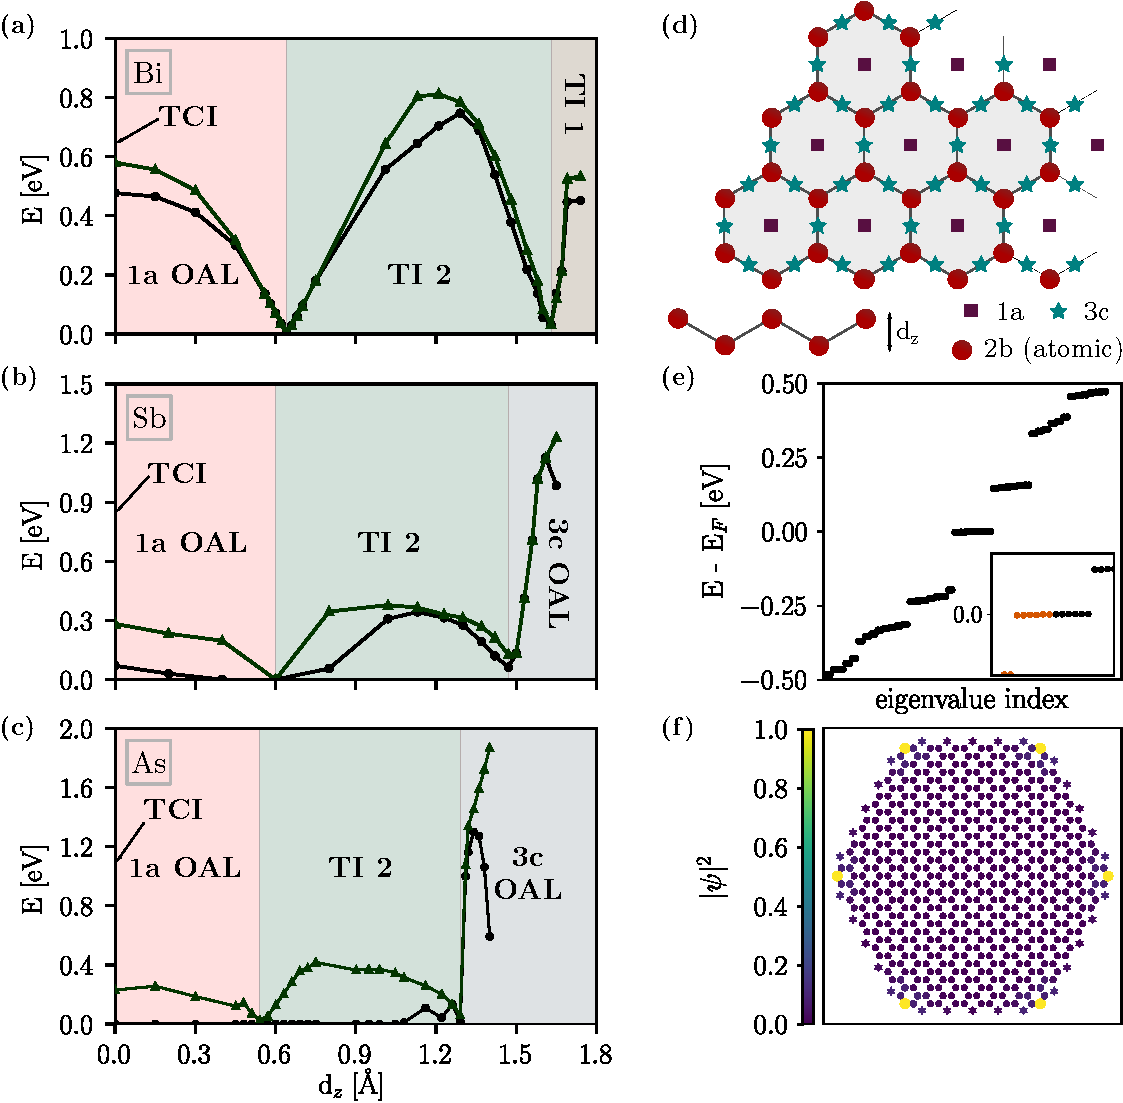
\includegraphics[width=\columnwidth]{oal_finite}
\caption{Low-energy spectrum of a finite armchair-terminated flakeof the 3cOAL. The inset presents the energies around the Fermi level, with filled states in orange. (f) The electronic densities of the cornerstates with color scale proportional to the normalized square modulus of the eigenstates $|\psi|^2$ (normalized with respect to the largest $|\psi|^2$).The tellurium atoms used for edge passivation are shown as stars.}
\label{fig:oal_finite}
\end{figure}


I\begin{table}[b]
	\centering
	\addtolength\tabcolsep{5pt}
	\begin{tabular}{|c||c|c|c|c|c|c||c||c|}
		\hline 
		phase & $\# \Gamma_2^{\mathcal{I}}$&  $\# M_2^{\mathcal{I}}$ & $[M^\mathcal{I}_2]$ & $\# \Gamma_2^{(3)}$ & $\# K_2^{(3)} $ & $[K^{(3)}_2]$  &  $\chi^{(3)}_{\mathcal{I}} = ([M^\mathcal{I}_2], [K^{(3)}_2])$ & $\Delta_{\textnormal{TI}}$ \\
\hline		
		TI 1 & 4 & 6 & 2 & 0 & 4 & 4  & (2, 4) & 1 \\
\hline 
		TI 2 & 4 & 6 & 2 & 2 & 4 & 2 & (2,  2) & 1 \\
		\hline 
		$3c$ OAL & 2 & 6 & 4 & 2 & 4 & 2  & (4, 2) & 0 \\
		\hline 
		$1a$ OAL & 4 & 4 & 0 & 2 & 4 & 2 & (0, 2) & 0\\
		\hline 
	\end{tabular} 
	\caption{\textbf{Topological invariants and symmetry indicators $\chi^{(3)}_{\mathcal{I}}$ corresponding to different regions in the phase diagrams:} The symmetry indicators were calculated using the primitive 2-site unit cell of the honeycomb lattice (see Table~\ref{tab:band_reps} for a decomposition in terms of elementary band representations). The indices $\chi^{(3)}_{\mathcal{I}}$ allow for a more refined classification even of the strong TIs. We find that the $3c$ and $1a$ OALs differ in their inversion indicator $[M^\mathcal{I}_2]$ and thus, as explained in the main text, inversion-symmetric flakes built from their hexagonal unit cells differ by a protected corner charge equal to $1 \mod 2$.}
	\label{tab:sym_indicators}	
\end{table}


We present the band representations of the space groups 164 (P$\bar{3}$m1) and 191 (P6/mmm) relevant for discussed materials. To deduce Wyckoff positions from which EBRs can be induced, we use data collected from the Bilbao Crystallographic Server~\cite{Aroyo2011183,Bilbao1, TQC2017, Vergniory17}. Note that we discard Wyckoff positions with nonzero $z$-component as they are irrelevant for a 2D geometry. The irreducible representations of bands at high-symmetry points were obtained using the \texttt{irrep} code~\cite{irrep-github}, which relies on the double space group character tables~\cite{elcoro2017} published on the Bilbao Crystallographic server~\cite{bilbao-server}.

\begin{table}[H]
	\centering
	\begin{tabular}{|c|c|c|c|}
		\hline 
		SG & phase & band representation & EBRs \\
		\hline
		164 & TI 1 & $(3\bar{\Gamma}_{8}\oplus 2\bar{\Gamma}_{9},2\bar{M}_{3}\bar{M}_{4}\oplus3\bar{M}_{5}\bar{M}_{6},2\bar{K}_{4}\bar{K}_{5}\oplus 3\bar{K}_{6})$ & -  \\
		\hline
		164 & TI 2 & $(2\bar{\Gamma}_{8}\oplus 2\bar{\Gamma}_{9}\oplus\bar{\Gamma}_{4}\bar{\Gamma}_{5},2\bar{M}_{3}\bar{M}_{4}\oplus3\bar{M}_{5}\bar{M}_{6},2\bar{K}_{4}\bar{K}_{5}\oplus 3\bar{K}_{6})$ & -  \\
		\hline
		164 & $3c$ OAL & $(3\bar{\Gamma}_{8}\oplus\bar{\Gamma}_{9}\oplus\bar{\Gamma}_{4}\bar{\Gamma}_{5},2\bar{M}_{3}\bar{M}_{4}\oplus3\bar{M}_{5}\bar{M}_{6},2\bar{K}_{4}\bar{K}_{5}\oplus 3\bar{K}_{6})$ &  $\bar{E}_{1}(2d)  \oplus\ {}^{1}\bar{E}_{g}^{2}\bar{E}_{g}(3c)  $  \\
		\hline
		164 & $1a$ OAL & $(2\bar{\Gamma}_{8} \oplus 2\bar{\Gamma}_{9} \oplus \bar{\Gamma}_{4} \bar{\Gamma}_{5}, 3 \bar{M}_3 \bar{M}_4 \oplus 2 \bar{M}_5 \bar{M_6}, 2 \bar{K}_4 \bar{K}_5 \oplus 3 \bar{K}_6)$ & $\bar{E}_{1g}(1a)  \oplus \bar{E}_{1u}(1a) \oplus \bar{E}_{1}(2d)  \oplus {}^{1}\bar{E}_{g}^{2}\bar{E}_{g}(1a) $ \\
		\hline \hline 
		191 & TCI  & $(\bar{\Gamma}_{7}\oplus \bar{\Gamma}_{8}\oplus\bar{\Gamma}_{9}\oplus\bar{\Gamma}_{11}\oplus \bar{\Gamma}_{12},3\bar{M}_{5}\oplus 2\bar{M}_{6},2\bar{K}_{7}\oplus \bar{K}_{8}\oplus 2\bar{K}_{9})$  & -  \\

		\hline
	\end{tabular} 
	\caption{Band representations corresponding to distinct phases as shown in Fig.~\ref{fig:materials} in the main text. `-' indicates that a given band representation cannot be written as a combination of EBRs.}
	\label{tab:band_reps}
\end{table}